\documentclass{article}
\usepackage{listings}
\usepackage{graphicx}
\usepackage{amsmath}

\begin{document}
\lstset{language=Pascal}          % Set your language (you can change the language for each code-block optionally)	
\title{Report of ...}
\author{Jialin Liu}
\date{\today}
\maketitle

\newpage

	\title{Project 1}
	\author{Jialin Liu \\ Tias \\ Thanaphong Phongpreecha}
	\maketitle
	
	\newpage
	
	\section{Introduction}
	Several differential equations can be written in a form of a non-homogeneous second-derivative differential equation 
	
	\begin{equation*}	
	\frac{d^{2}y}{dx^2} + k^2(x)y=f(x)
	\end{equation*}
	
	This equation is versatile and is encountered in many fields. For example in engineering, it could be used for modeling mechanical and electrical oscillators with external force. \cite{example}
	
	The goal of this project is to use computational calculations, if possible, with dynamic memory allocation to solve the one-dimensional Poisson's equation in electromagnetism with Dirichlet boundary conditions. Detailed derivation can be found in the problem statement, but essentially, the 3D Poisson's equation is simplified to 1D (radial dimension) based on its spherical symmetry. After simplifying to 1D, the differential equation is discretized by rewriting to a set of linear equations of,
	
	\begin{align*}
	-\frac{v_{i+1}+v{i-1}-2v_i}{h^2}=f_i && \text{for i = 1,...,n}
	\end{align*}
	The equation is solved by transforming to a tridiagonal matrix with $f(x)=100 \cdot e^{-10x}$, where $x \in (0,1) $. These matrices can then be solved using conventional techniques, such as Gaussian Elimination and LU Decomposition \cite{rice2012applied}. The results will be compared with exact solution given as $u(x)=1-(1-e^{10})x-e^{-10x}$. The analyses of results generated in this report include, in an order of,
	
	\begin{enumerate}
		\item the contribution of the number of steps $h$ to the accuracy of the estimation as compared to exact results 
		\item the relative errors of different step length 
		\item the differences and limits in using either LU decomposition or Gaussian Elimination approach to solve the matrix
		\item the analytic solutions to this particular problem, and 
		\item the differences in computing time by MATLAB, Python, and Fortran using the same laptop.
		
	\end{enumerate}
	
	
	
\section{Theoretical models and technicalities}
\subsection{Gaussian Elimination for Tridiagonal Matrix}	
To solve ordinary differential equation, Central Euler method is commonly used to achieve $o(h^2)$ accuracy as shown in Eq.1 for second order derivative:\\

\begin{align}
\frac{x_{i+1}+x_{i-1}-2*x_i}{h^2} = f{''}_i,
\end{align}

where h is the step length, $x(i)$ is the $i^th$ points and $f$ is the function value at the $i^th$ point. \\
This method can be implemented to solve many ODEs involving first and second order derivatives in the following form numerically:\\

\begin{align}
\frac{d^2y}{dx^2}+k^2(x)y = f(x),
\end{align}

where $k^2$ is a real function.\\
For example, for the Poission's equation under spherical symmetrical field using polar coordinations, the original equation can be simplified as following form:\\

\begin{align}
\frac{1}{r^2}\frac{d}{dr}\left(r^2\frac{d\Phi}{dr}\right) = -4\pi \rho(r),
\end{align}

where $\phi$ is the electrostatic potential, $\rho(r)$ is the local charge distribution and $r$ is the radial distance\\
If we substitute $\Phi(r)= \phi(r)/r$, we can have \\

\begin{align}
\frac{d^2\phi}{dr^2}= -4\pi r\rho(r).
\end{align}

by letting $\phi\rightarrow u$ and $r\rightarrow x$, this equation can be transformed into a simple form:

\begin{align}
-u''(x) = f(x). 
\end{align}

After discretizing this function on the region of $(0, 1)$, at each point $x_i$, Central Eular method can be used to calculate the second order derivative. At the $i^th$ point, the function value of Poisson Equation can be approximate using:

\begin{align}
   -\frac{v_{i+1}+v_{i-1}-2v_i}{h^2} = f_i  \hspace{0.5cm} \mathrm{for} \hspace{0.1cm} i=1,\dots, n,
\end{align}

We rewrite this equation as a linear equation system into the form of

\begin{align}
{\bf A}{\bf v} = \tilde{{\bf b}},
\end{align}

where ${\bf A}$ is an $n\times n$  tridiagonal matrix which we rewrite as 
\begin{equation}
{\bf A} = \left(\begin{array}{cccccc}
2& -1& 0 &\dots   & \dots &0 \\
-1 & 2 & -1 &0 &\dots &\dots \\
0&-1 &2 & -1 & 0 & \dots \\
& \dots   & \dots &\dots   &\dots & \dots \\
0&\dots   &  &-1 &2& -1 \\
0&\dots    &  & 0  &-1 & 2 \\
\end{array} \right)
\end{equation}
and $\tilde{b}_i=h^2f_i$.\\

In this special matrix, the $o(n^3)$ Gaussian Elimination (GE) methods can be simplified to Tridiagonal Gaussian Elimination (TGE) method which cost only $o(8n)$ floating point calculations.

In the standard GE method, when we eliminate the first row, $A_{21}$ will be eliminated and so will all $A_{i,i-1}$ elements. Then let's consider elimination of the  $i^th$ row. The element on diagonal is $A_{i,i}$. The element on the left of diagonal, $A_{i,i+1}$ will remain 0 after elimination because the elements above it are all 0. After forward substitution, all $A_{i,i-1}$ elements are 0 and all $A_{i,i+1}$ elements are -1. All elements on diagonal,$d_i$, will be substitute to a new value, $\tilde{{d_i}}$. \\
If we add $N$ extra points in $(0,1)$, the matrix $A$ will be a N by N matrix. After forward substitution, the $N^th$ row have only one element, $A_{N,N}$ so the corresponding function value,$u_{N}$, can be solved easily. For the $i^th$ row, if we expand the matrix operation, we will have the following equation:

\begin{align}
\tilde{{A_{i,i}}}*u_i-u_{i+1} = \tilde{f_i},
\end{align}

where $u_i$ is the approximated function value at $i^th$ point.Since $u_{i+1}$ is already solved from previous step, the $u_i$ can also solved from this equation. In this TGE method, only 8N FLOPS are needed to solve for N points.\\
Assume
\begin{align}
f(x) = 100e^{-10x},
\end{align}
and we can get the closed form solution:

\begin{align}
u(x) = 1-(1-e^{-10})x-e^{-10x}
\end{align}

So, the relative error in each point can be calculated as 

\begin{align}
   \epsilon_i=log_{10}\left(\left|\frac{v_i-u_i}
   {u_i}\right|\right),
\end{align}
where $u_i$ is the exact solution and $v_i$ is the numerical solution.

\subsection{LU decomposition}
In LU decomposition method, a matrix $A$ can be decomposed into the product of two special matrices,$L$ and $U$ which is shown below:

\begin{align}
A = L*U,
\end{align}

where L is a lower triangle matrix with all diagonal elements as 1 and U is a upper triangle matrix. LU decomposition required $o(N^3)$ floating points calculation which is same as standard GE method. However, after LU decomposition, the determinate can be easily calculated as product of diagonal elements in U matrix.

\subsection{Implement TGE in Codes}

To compare the calculation speed of different methods and efficiency of different programming languages, TGE and LU method are implemented in Matlab and Python to solve the Poisson Equation under Dirichlet boundary conditions on the region of $(0, 1)$ using 10, 100, 1000 and 10000 points.
\subsubsection{Matlab}
MATLAB is a high-level language and interactive environment for numerical computation, visualization, and programming. MATLAB can analyze data, develop algorithms, and create models and applications. The language, tools, and built-in math functions can be used to explore multiple approaches and reach a solution faster than with spreadsheets or traditional programming languages, such as C/C++ or Java. Also, MATLAB can be used for a range of applications, including signal processing and communications, image and video processing, control systems, test and measurement, computational finance, and computational biology. More than a million engineers and scientists in industry and academia use MATLAB, the language of technical computing. \\
Matlab is specifically expertise on matrix operation, the first part of Matlab program simply called the native slash operator to solve Poission equation:\\
 \begin{lstlisting}[frame=single]  
Matlab_cal_u = (f/A);
 \end{lstlisting}
 
 The TGE method is implemented using FOR loop to ensure the using of atomic operation in Matlab. All variables are initialized at the beginning of this program based on different number of data points. In the backward subsitution, the last row is calculated separately and then other rows are calculated in a FOR loop.
  \begin{lstlisting}[frame=single]  
% Forward Subsitute
for i = 2:size(A,1)
	ratio = -(A(i,i-1)/A(i-1,i-1));
	A(i,:) = A(i,:)+A(i-1,:)*ratio;
	f(i) = f(i)+f(i-1)*ratio;
end

% Backward Subsitue
cal_u(N-2) = f(N-2)/A(N-2,N-2);
for i = (size(A,1)-1):-1:1
	cal_u(i) = (f(i)-cal_u(i+1)*A(i,i+1))/(A(i,i));
end
  \end{lstlisting}
  
  For the LU decomposition, a native lu() function is used to calculate the two matrices and the slash operator is used on each matrix to solve function value:\\
  \begin{lstlisting}[frame=single]  
[L,U] = lu(fullMatrix);
LU_results = (f0/L)/U;
  \end{lstlisting}  
  One thing to be notice is, in Matlab, the efficiency of FOR loop is relatively low comparing with matrix operation. To assign value for each element in the matrix, extra floating point calculations are needed.
\subsubsection{Python}
Python is an easy to learn, powerful programming language. It has efficient high-level data structures and a simple but effective approach to object-oriented programming. Python’s elegant syntax and dynamic typing, together with its interpreted nature, make it an ideal language for scripting and rapid application development in many areas on most platforms.
Comparing with Matlab, similar data structure and algorithms are used in Python code. Also numpy package and scipy.linalg module are used for mathematical operations and matplotlib is used for graph plotting. The core code for TGE is shown below:
  \begin{lstlisting}[frame=single]  
# Forward Substitution
for i in xrange(1, n-1):
d[0, i] = d[0, i] - e[0, i-1] / d[0, i-1] * e[0, i-1]
f[i] = f[i] - e[0, i-1] / d[0, i-1] * f[i-1]
# Backward Substitution
u[0, n-2] = f[n-2] / d[0, n-2]
for i in range(n-3, -1, -1):
u[0, i] = (f[i] - e[0, i] * u[0, i+1]) / d[0, i]
  \end{lstlisting}  
  And for the LU decomposition, 
    \begin{lstlisting}[frame=single]  
    LU = la.lu_factor(A)
    X = la.lu_solve(LU, f)
    \end{lstlisting} 
------------------------------------------------------------------------------------------------------
------------------------------------------------------------------------------------------------------
------------------------------------------------------------------------------------------------------
------------------------------------------------------------------------------------------------------
------------------------------------------------------------------------------------------------------

\subsection{General Results}

The primary goal of this project is to obtain numerical solution for one dimensional Poisson's equation. The results as shown in Figure \ref{fig:NumSoln_Matlab} validates that the result for inhomogeneous second-order differential equation can be approximated by transforming to set of linear equations. A reliable approximation ($u$), as compared to exact solution ($u_{exact}$) can be achieved by using steps of more than 100. Detail on accuracy and errors will be discussed in the next section. Solving the matrices either by Gaussian elimination or LU decomposition yielded the same exact results as they should be.

\begin{figure}[h]
\centering
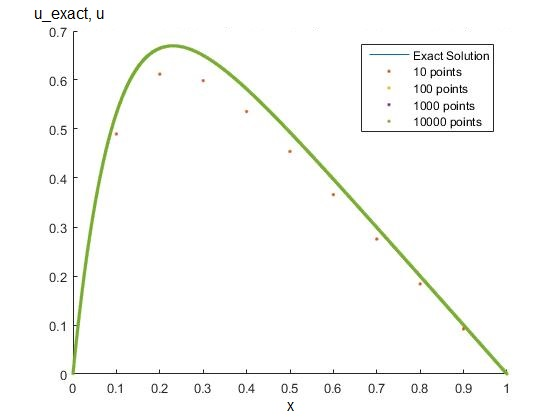
\includegraphics[width=1\linewidth]{../figures/NumSoln_Matlab}
\caption{Exact solution ($u_{exact}$) and estimates $u$ from solving the set of linear equations by using different number of points.}
\label{fig:NumSoln_Matlab}
\end{figure}


\subsection{Errors in Approximations}

\begin{figure}[h]
\centering
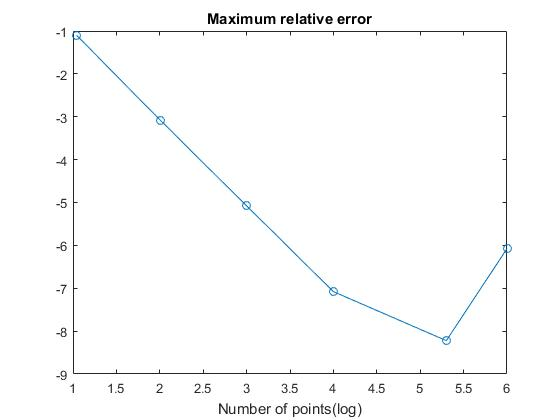
\includegraphics[width=1\linewidth]{../figures/Err_Matlab}
\caption{Relative error by using different no. of points in Gaussian elimination method.}
\label{fig:Err_Matlab}
\end{figure}

The error presented in both LU decomposition and Gaussian elimination methods are the same as plotted in Figure \ref{fig:Err_Matlab}. The plot is from Gaussian elimination because LU decomposition of size larger than 10,000 step size consumes excessed amount of memories and cannot be compiled on our computers.

Generally, the error decreases as step size increases. However, there is a limitation to the accuracy and caution should be paid when using this estimation. We found that at certain step size between 200,000 and 1,000,000, the trend reverses. This starts as early as 500,000 (tested, but not shown). The growing errors are most likely stemmed from the rounding error -- as the step sizes got too small. 


\begin{figure}[H]
	\centering
	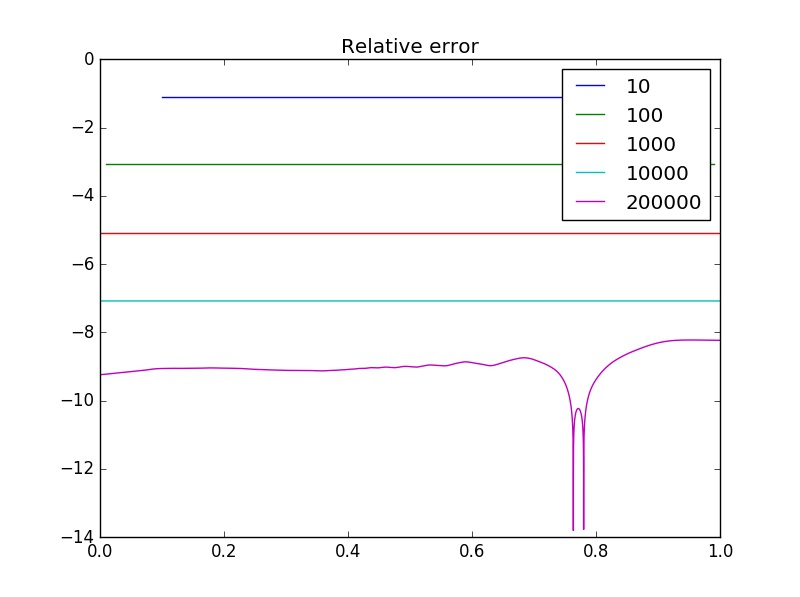
\includegraphics[width=1\linewidth]{../figures/Err_Python_200k}
	\caption{Relative error of different step sizes as a function of x.}
	\label{fig:Err_Python_200k}
\end{figure}

To delve deeper in to this issue, a separate plot of the relative errors along x of different step size was generated (Figure \ref{fig:Err_Python_200k}). From this graph, we found that the error from step sizes of 10-10000 are negligible. However, starting as soon as 200,000 points the results begin to fluctuate. Although at this point it still follow the decreasing trend in error shown in Figure \ref{fig:Err_Matlab}, this marks a beginning of instability.



	\bibliographystyle{plain}
	\bibliography{Reference}
	
\end{document}
